\documentclass[twocolumn]{aastex63}

% typography
\usepackage[T1]{fontenc}
\usepackage{times}
\usepackage{bm}

\setlength{\parindent}{1.\baselineskip}
\newcommand{\acronym}[1]{{\small{#1}}}
\newcommand{\package}[1]{\textsl{#1}}
\newcommand{\gaia}{\textsl{Gaia}}
\newcommand{\jwst}{\textsl{JWST}}
% \newcommand{\pans}{\textsl{Pan-STARRS}}

% \newcommand{\deg}{\ensuremath{\textrm{deg}}}
\newcommand{\msun}{\ensuremath{\textrm{M}_\odot}}
\newcommand{\myr}{\ensuremath{\textrm{Myr}}}
\newcommand{\gyr}{\ensuremath{\textrm{Gyr}}}
\newcommand{\kpc}{\ensuremath{\textrm{kpc}}}
\newcommand{\pc}{\ensuremath{\textrm{pc}}}
\newcommand{\kms}{\ensuremath{\textrm{km}\,\textrm{s}^{-1}}}
\newcommand{\masyr}{\ensuremath{\textrm{mas}\,\textrm{yr}^{-1}}}
\newcommand{\feh}{\ensuremath{\textrm{[Fe/H]}}}
\newcommand{\afe}{\ensuremath{\textrm{[$\alpha$/Fe]}}}
\newcommand{\changes}[1]{{\textbf{#1}}}
\hyphenation{kruijs-sen}

% aastex parameters
% \received{not yet; THIS IS A DRAFT}
%\revised{not yet}
%\accepted{not yet}
% % Adds "Submitted to " the argument.
% \submitjournal{ApJ}
\shorttitle{}
\shortauthors{bonaca \& kruijssen}

%@arxiver{}
\usepackage{amsmath}

\begin{document}\sloppy\sloppypar\raggedbottom\frenchspacing % trust me

\title{The Progenitor Globular Clusters of Stellar Streams in the Galactic Halo}

\correspondingauthor{Ana~Bonaca}
\email{ana.bonaca@cfa.harvard.edu}

\author[0000-0002-7846-9787]{Ana~Bonaca}
\affil{Center for Astrophysics | Harvard \& Smithsonian, 60 Garden Street, Cambridge, MA 02138, USA}

\author[0000-0002-8804-0212]{J.~M.~Diederik~Kruijssen}
\affiliation{Astronomisches Rechen-Institut, Zentrum f\" ur Astronomie der Universit\" at Heidelberg, M\" onchhofstra\ss e 12-14, D-69120 Heidelberg, Germany}
\affil{Center for Astrophysics | Harvard \& Smithsonian, 60 Garden Street, Cambridge, MA 02138, USA}


\begin{abstract}\noindent % trust me
We present orbits and masses of 22 thin stellar streams in the Milky Way.
We constrain the streams' orbits by fitting the combined 5D phase-space of sky positions, distances and proper motions, including radial velocities where available.
Assuming that the streams are globular clusters that tidally evaporated in 10\,Gyr, we use orbital apocenters and eccentricities to estimate their pre-evaporation masses.
Beyond a galactocentric radius of $\sim10$~kpc, fossil streams follow a similar distribution of orbital apocenters as the surviving globular clusters, but have somewhat lower orbital eccentricities.
Strikingly, their pre-evaporation masses are more than an order of magnitude lower, with a median of $8.5\times10^3\,\msun$.
The progenitors of tidal streams observed at present are a specific, low-mass subset of the initial globular cluster population.
Building on these findings, we conclude that (1) globular clusters represent the high-mass end of a broader initial cluster population extending into the low-mass regime of clusters observed to form today,
(2) the internal dynamics plausibly had a limited role in sculpting the observed density variations in streams such that external perturbations (e.g., from dark-matter subhalos) are required, and
(3) the progenitor clusters of the lowest-metallicity stellar streams may have constituted a significant fraction of their host galaxy's mass at the time of their formation.
% 208 words; victory
\end{abstract}

\section{Introduction}
\label{sec:intro}

Unveiling the origin of the ancient globular clusters remains a major challenge in modern astrophysics \citep[e.g.][]{brodie:2006,kruijssen:2014,renaud:2017,forbes:2018,adamo:2020}.
Broadly speaking, the field is divided into two families of models.
The first interprets globular clusters as the products of unique conditions that exist mostly or exclusively in the early Universe \citep[e.g.][]{peebles:1968,fall:1985,ashman:1992,trenti:2015,madau:2020}.
% In recent years, a second interpretation has been gaining traction, which is that globular clusters are the natural outcome of regular star formation in normal high-redshift galaxies \citep[e.g.][]{kravtsov:2005,kruijssen15b,pfeffer:2018,keller:2020}.
In recent years, a second interpretation has been gaining traction, which is that globular clusters are the natural outcome of regular star formation in high-redshift galaxies \citep[e.g.][]{kravtsov:2005,kruijssen15b,pfeffer:2018,keller:2020}.
% Both scenarios predict vastly different globular cluster formation histories at high redshifts.
\changes{These} scenarios predict vastly different globular cluster formation histories at high redshifts\changes{: the former predicts that most globular clusters formed were massive and survived to the present, while the latter predicts a large population of disrupted low-mass globular clusters}.
Most globular clusters are old \citep[$\gtrsim10\,\gyr$,][]{marinfranch09, dotter10, dotter11, vandenberg13, leaman:2013}, and their ages are notoriously imprecise, but demographics of young proto-globular clusters observed directly at high redshift could potentially distinguish between these ideas \citep[e.g., with the upcoming \textsl{James Webb Space Telescope}, \jwst,][]{gardner:2006}.
However, this experiment is greatly complicated by the fact that the current population of globular clusters represents the `tip of the iceberg' that survived nearly a Hubble time of dynamical evolution and disruption.
It is not clear how to connect the current globular cluster population to the initial one.

Theoretical studies of the dynamics of globular clusters orbiting in the Galactic halo predict that stars escape globular clusters due to two-body relaxation and tidal stripping \citep[often referred to as `evaporation', e.g.,][]{spitzer:1987, baumgardt03}, forming long and thin tidal tails along the cluster's orbit \citep{combes:1999}.
Such tidal tails were first detected around the Palomar~5 globular cluster \citep{odenkirchen:2001, rockosi:2002}.
Stellar streams of similar width and length, but without a surviving progenitor, have been discovered throughout the Milky Way \citep[e.g.,][]{gd:2006, grillmair:2009, bonaca:2012, balbinot:2016, bernard:2016, shipp:2018, malhan:2018, ibata:2019, caldwell:2020}.
Measurements of a small metallicity dispersion in some of these streams indicate that they likely constitute a population of completely dissolved globular clusters \citep{li:2017,bonaca:2020b, hansen:2020, ji:2020}.

The two families of globular cluster formation models predict qualitatively different initial globular cluster mass functions.
Reconstructing masses of stellar stream progenitors at the onset of the evaporation process that led to their dissolution would help distinguish these formation channels.
Models relying on unique, early-universe conditions often predict that globular clusters are born with a characteristic mass scale related to the conditions of their formation \citep[e.g.][]{peebles:1968,fall:1985,trenti:2015,madau:2020}.
This translates into the characteristic mass scale of $\sim10^5~\msun$ observed in the present-day globular clusters without requiring the prevalent disruption of lower-mass clusters.
In this family of models, one would expect the masses of fossil stream progenitors to be similar to those of globular clusters.

By contrast, models that describe globular clusters as the outcomes of regular star and cluster formation generally assume that their initial mass distribution followed a power law with an index around $-2$, mirroring observations of young cluster populations in the local Universe \citep[e.g.,][]{larsen:2009,adamo:2020}.
This power law mass distribution then evolves into the current, peaked form by dynamical disruption of low-mass clusters due to early tidal perturbations in the natal galaxy and subsequent evaporation in the halo \citep{elmegreen:1997,fall:2001,elmegreen:2010,kruijssen15b}.
\changes{clarify natal can be main mw progenitor}
This scenario predicts the existence of a population of low-mass clusters that vanished by dynamical disruption.
Because globular cluster disruption proceeds more rapidly at low masses \citep{baumgardt03,krumholz:2019}, the progenitor clusters of stellar streams may have been part of this putative low-mass cluster population.
In this family of models, one would expect the masses of fossil stream progenitors to be lower than those of globular clusters.

Our goal in this paper is to estimate masses of disrupted globular clusters that are now observed as stellar streams in the Milky Way.
Progenitor masses have already been estimated for several streams based on their widths \citep{erkal:2016b, erkal:2016, shipp:2018}, however, under the assumption that the streams are on circular orbits in a spherical gravitational potential.
In this work we take a different approach and derive an expression for the cluster's pre-evaporation mass that fully accounts for its orbit.
The timescale for cluster evaporation is determined by: (1) its initial mass, i.e.\ more massive clusters survive over longer timescales, and (2) its orbit, i.e.\ clusters on more eccentric orbits and with smaller apocenters dissolve faster \citep{baumgardt03,kruijssen09}.
This means that the pre-evaporation masses of stellar streams can be estimated by determining their orbits and assuming an age.
\changes{.}
Velocities are essential for accurately estimating the streams' orbits \citep{bh:2018}, and thanks to Gaia proper motions \citep{gdr2}, there are now 22 stellar streams with known kinematics, making it feasible to carry out the proposed exercise.

The structure of this paper is as follows.
In Section~\ref{sec:orbits} we use the observed positions and motions of stream stars to determine their orbits.
Since the streams are thin and coherent, we assume that the progenitors are globular clusters (and not dwarf galaxies) that disrupted recently \citep{helmi:2003}, and in Section~\ref{sec:disrupted} calculate their pre-evaporation masses.
We place this population of disrupted globular clusters in the context of cluster formation (\S\,\ref{sec:discuss_gcform}), discuss the implications of the inferred low masses for streams as dynamical tracers in the Milky Way halo (\S\,\ref{sec:discuss_dynamics}), and connect the cluster properties to those of the host galaxies they might have formed in at high redshift (\S\,\ref{sec:discuss_galform}).

\section{Stream Observations}
\label{sec:obs}

Several dozen of thin stellar streams, likely disrupted globular clusters, have been reported in the Milky Way \citep[an up-to-date list is available in the \package{galstreams} package,][]{mateu:2018}.
Because kinematic information is essential for accurate stream modeling \citep{bh:2018}, here we limit our analysis to 22 stellar streams with published proper motions.

Tidal debris from evaporating globular clusters nearly delineates the progenitor's orbit \citep[e.g.,][]{dehnen:2004, koposov:2010, kupper:2012}.
We use the observed sky positions, distances, proper motions, and, where available, radial velocities to find the streams' orbits.
Member stars have been identified along most streams in our sample, so for those we use their phase-space coordinates directly.
For the most diffuse streams (Ravi, Turbio, Wambelong, and Willka-Yaku), only average distances and proper motions are available \citep{shipp:2019}, so we distribute 20 control points between these streams' endpoints \citep{riley:2020}, and assume that distance and proper motion are constant along the stream.
The complete provenance of the original measurements is described in Appendix~\ref{sec:appendix} and summarized in Table~\ref{table:phasespace}.
All of the data points we used to fit are available in the project repository\footnote{\url{https://github.com/abonaca/disrupted_gc}}.
An example is presented in Figure~\ref{fig:streams}. On the left side of Figure~\ref{fig:streams} we show (from the top) the observed sky positions, distances, and components of the proper motion vector for the Fj\" orm stream as orange points.
The interactive version of this Figure contains a gallery of all the streams in our sample and is available in the online version of this article, and \href{https://www.cfa.harvard.edu/~abonaca/stream_gallery/gallery.html}{here}.

\begin{figure*}
\begin{center}
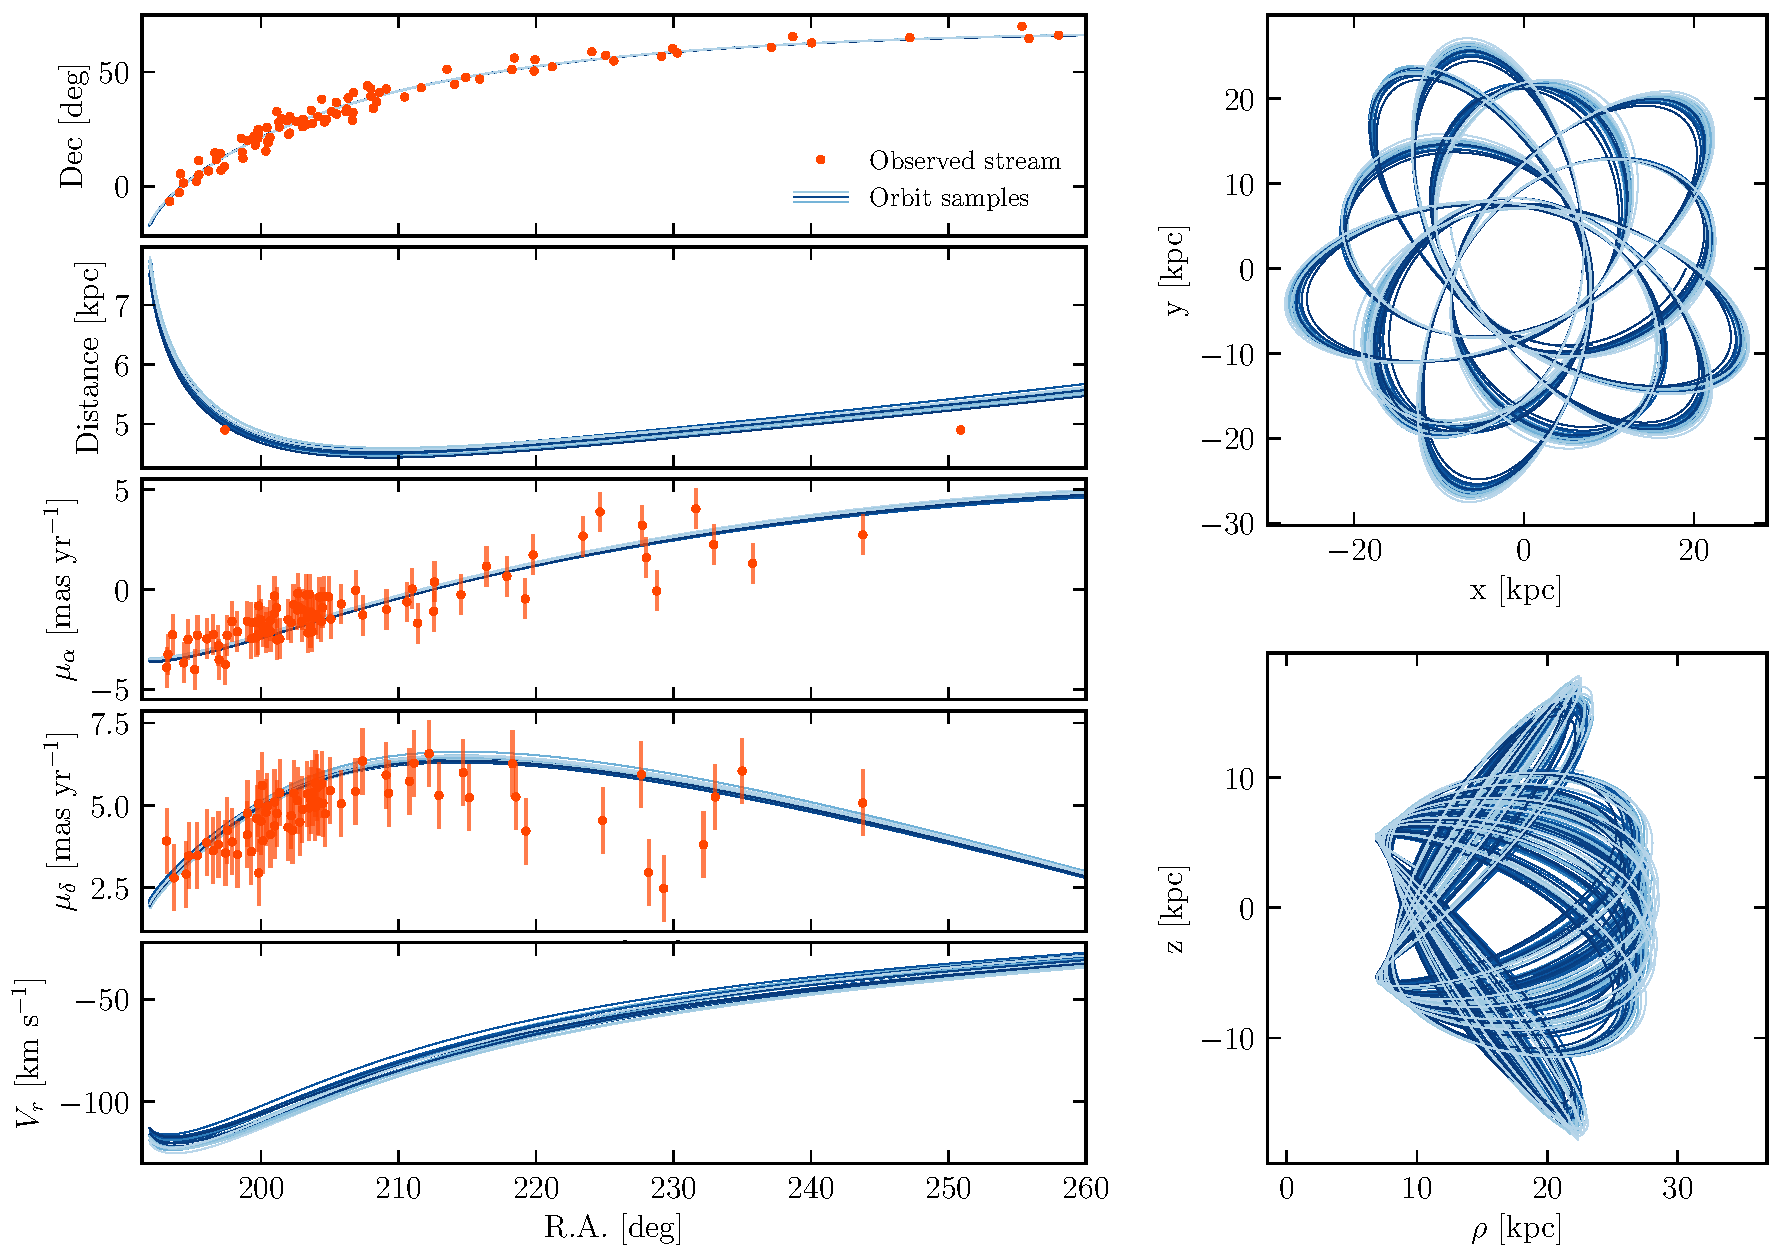
\includegraphics[width=0.9\textwidth]{stream_fitting.pdf}
\end{center}
\caption{Orbital constraints for the Fj\"{o}rm stellar stream in the observed coordinates (left: panels from top to bottom show declination, distance, proper motion components and radial velocity as a function of right ascension) and cylindrical Galactocentric coordinates (right: in and out of the Galactic plane for the top and bottom panels, respectively).
Different shades of blue represent orbit samples from the posterior constrained by the stream observations (orange points).
Current observations allow for a range of orbital apocenters and eccentricities.
}
\label{fig:streams}
\end{figure*}


\section{Stream Orbits}
\label{sec:orbits}

\begin{deluxetable}{l @{\hspace{0.5cm}} D D D}
\tablehead{
Name & \multicolumn2c{$r_{\rm peri}$} & \multicolumn2c{$r_{\rm apo}$} & \multicolumn2c{$\log M_0/\rm\msun$}\\
& \multicolumn2c{kpc} & \multicolumn2c{kpc} & \multicolumn2c{dex}
}
\decimals
\setlength{\tabcolsep}{3pt}
\startdata
ATLAS & $30.7$ & -33.2$^{+0.2}_{-0.2}$ & 21.7$^{+3.0}_{-3.0}$ & -0.1$^{+0.5}_{-0.5}$ & -0.7$^{+0.2}_{-0.2}$ & 96.7$^{+87.7}_{-96.9}$ & 17.7$^{+5.0}_{-5.2}$ & 32.3$^{+22.7}_{-7.0}$ & $3.61\pm0.19$ \\ 
Aliqa Uma & $40.6$ & -38.3$^{+0.2}_{-0.2}$ & 27.6$^{+3.6}_{-3.7}$ & 0.2$^{+0.4}_{-0.4}$ & -0.2$^{+0.3}_{-0.3}$ & 147.8$^{+155.2}_{-173.4}$ & 17.8$^{+8.5}_{-5.9}$ & 48.3$^{+65.2}_{-15.6}$ & $3.49\pm0.25$ \\ 
Chenab & $-28.3$ & -43.0$^{+0.5}_{-0.5}$ & 39.1$^{+5.0}_{-4.8}$ & -0.1$^{+0.2}_{-0.2}$ & -2.5$^{+0.4}_{-0.5}$ & 27.0$^{+103.6}_{-111.5}$ & 28.6$^{+6.9}_{-11.4}$ & 63.9$^{+73.3}_{-26.2}$ & $3.23\pm0.32$ \\ 
Elqui & $20.6$ & -42.4$^{+0.3}_{-0.3}$ & 48.6$^{+6.2}_{-6.1}$ & -0.1$^{+0.3}_{-0.3}$ & -0.3$^{+0.2}_{-0.2}$ & 98.4$^{+160.2}_{-155.8}$ & 33.3$^{+12.8}_{-14.3}$ & 91.4$^{+98.8}_{-35.3}$ & $3.08\pm0.30$ \\ 
Fimbulthul & $214.2$ & -22.6$^{+0.3}_{-0.3}$ & 4.2$^{+0.0}_{-0.0}$ & -15.1$^{+0.3}_{-0.3}$ & -10.1$^{+0.4}_{-0.4}$ & 74.6$^{+1.9}_{-1.8}$ &  1.5$^{+0.1}_{-0.1}$ &  7.1$^{+0.1}_{-0.1}$ & $5.10\pm0.05$ \\ 
Fj\"{o}rm & $197.4$ & 5.6$^{+0.4}_{-0.4}$ & 4.9$^{+0.0}_{-0.1}$ & -3.7$^{+0.2}_{-0.3}$ & 3.9$^{+0.4}_{-0.4}$ & -113.0$^{+8.8}_{-8.5}$ &  8.2$^{+0.0}_{-0.0}$ & 24.0$^{+3.0}_{-2.9}$ & $4.03\pm0.03$ \\ 
Gj\"{o}ll & $70.2$ & -2.6$^{+0.3}_{-0.3}$ & 3.5$^{+0.1}_{-0.1}$ & 22.1$^{+0.5}_{-0.5}$ & -22.9$^{+0.5}_{-0.5}$ & -25.8$^{+11.8}_{-11.2}$ &  9.3$^{+0.2}_{-0.2}$ & 29.6$^{+3.6}_{-3.0}$ & $3.93\pm0.03$ \\ 
Indus & $-36.3$ & -50.7$^{+0.6}_{-0.6}$ & 16.5$^{+1.8}_{-1.6}$ & 2.6$^{+0.4}_{-0.3}$ & -5.9$^{+0.5}_{-0.6}$ & 4.4$^{+64.6}_{-71.6}$ & 11.7$^{+2.1}_{-3.1}$ & 28.2$^{+30.8}_{-11.6}$ & $3.85\pm0.23$ \\ 
Leiptr & $61.0$ & 0.7$^{+0.3}_{-0.3}$ & 8.3$^{+0.3}_{-0.2}$ & 8.9$^{+0.4}_{-0.4}$ & -10.1$^{+0.5}_{-0.5}$ & -84.0$^{+18.3}_{-18.8}$ & 12.8$^{+0.4}_{-0.4}$ & 45.4$^{+14.3}_{-10.8}$ & $3.68\pm0.07$ \\ 
Phoenix & $20.1$ & -55.3$^{+0.1}_{-0.1}$ & 18.5$^{+1.7}_{-1.4}$ & 2.8$^{+0.3}_{-0.3}$ & 0.3$^{+0.5}_{-0.4}$ & 115.6$^{+107.1}_{-118.6}$ & 12.1$^{+5.1}_{-4.5}$ & 26.3$^{+18.1}_{-6.1}$ & $3.84\pm0.20$ \\ 
Ravi & $-16.0$ & -59.6$^{+0.5}_{-0.5}$ & 21.7$^{+3.2}_{-3.0}$ & 0.6$^{+0.3}_{-0.2}$ & -1.0$^{+0.4}_{-0.3}$ & 148.3$^{+71.6}_{-81.7}$ &  7.1$^{+3.7}_{-2.6}$ & 21.2$^{+4.2}_{-2.9}$ & $4.12\pm0.20$ \\ 
Slidr & $178.0$ & 3.3$^{+0.4}_{-0.3}$ & 3.4$^{+0.1}_{-0.1}$ & -25.5$^{+0.6}_{-0.6}$ & -3.6$^{+0.3}_{-0.3}$ & 78.5$^{+9.1}_{-9.1}$ &  2.4$^{+0.3}_{-0.3}$ & 27.2$^{+2.1}_{-1.9}$ & $4.65\pm0.07$ \\ 
Sv\"{o}l & $244.4$ & 23.5$^{+0.3}_{-0.4}$ & 8.1$^{+0.1}_{-0.2}$ & -4.4$^{+0.1}_{-0.1}$ & -0.9$^{+0.2}_{-0.2}$ & -109.0$^{+4.8}_{-5.4}$ &  1.0$^{+0.1}_{-0.1}$ &  8.7$^{+0.1}_{-0.2}$ & $5.27\pm0.04$ \\ 
Sylgr & $186.6$ & -0.8$^{+0.3}_{-0.3}$ & 4.1$^{+0.0}_{-0.0}$ & -18.7$^{+0.4}_{-0.4}$ & -13.5$^{+0.3}_{-0.3}$ & 54.5$^{+4.3}_{-4.7}$ &  5.3$^{+0.3}_{-0.2}$ & 14.1$^{+0.9}_{-0.8}$ & $4.34\pm0.03$ \\ 
Tucana III & $3.2$ & -59.4$^{+0.1}_{-0.1}$ & 24.5$^{+3.0}_{-2.7}$ & -0.3$^{+0.4}_{-0.5}$ & -1.8$^{+0.2}_{-0.2}$ & 178.9$^{+209.1}_{-236.5}$ & 11.9$^{+6.4}_{-6.9}$ & 39.8$^{+57.4}_{-15.2}$ & $3.76\pm0.36$ \\ 
Turbio & $27.9$ & -48.3$^{+1.3}_{-1.8}$ & 16.9$^{+1.3}_{-0.8}$ & 2.1$^{+0.1}_{-0.2}$ & -5.2$^{+1.1}_{-0.9}$ & 68.6$^{+2.9}_{-3.6}$ & 14.5$^{+2.5}_{-5.8}$ & 33.0$^{+79.6}_{-12.8}$ & $3.69\pm0.34$ \\ 
Turranburra & $75.2$ & -26.3$^{+0.4}_{-0.4}$ & 26.9$^{+3.7}_{-3.9}$ & 0.1$^{+0.4}_{-0.4}$ & -0.4$^{+0.2}_{-0.2}$ & 195.8$^{+85.5}_{-111.2}$ & 15.8$^{+9.2}_{-7.3}$ & 38.7$^{+19.6}_{-5.1}$ & $3.60\pm0.28$ \\ 
Wambelong & $79.3$ & -34.4$^{+0.3}_{-0.3}$ & 16.2$^{+1.6}_{-1.4}$ & 2.2$^{+0.2}_{-0.2}$ & -1.4$^{+0.3}_{-0.4}$ & 263.0$^{+32.0}_{-43.0}$ &  2.4$^{+1.5}_{-0.7}$ & 22.6$^{+1.8}_{-1.5}$ & $4.67\pm0.22$ \\ 
Willka Yaku & $36.1$ & -64.6$^{+0.2}_{-0.1}$ & 34.5$^{+3.7}_{-3.1}$ & 1.3$^{+0.1}_{-0.1}$ & 0.7$^{+0.4}_{-0.3}$ & 196.1$^{+173.2}_{-201.3}$ & 22.0$^{+10.5}_{-10.2}$ & 76.1$^{+87.2}_{-34.1}$ & $3.33\pm0.29$ \\ 
Ylgr & $169.1$ & -10.4$^{+0.3}_{-0.3}$ & 9.4$^{+0.2}_{-0.2}$ & -0.6$^{+0.2}_{-0.3}$ & -8.2$^{+0.5}_{-0.6}$ & 147.7$^{+13.3}_{-13.8}$ &  7.7$^{+0.7}_{-0.7}$ & 18.4$^{+3.5}_{-2.5}$ & $4.11\pm0.07$ \\ 

\enddata
\caption{Derived properties of stellar streams: orbital pericenter, apocenter and the pre-evaporation mass of the stream's progenitor.
Quoted values are the medians of the sampled posterior distributions and the uncertainties reflect their $16-84$ percentiles.
The second set of mass uncertainties are systematic between different Milky Way models.
}
\label{table:constraints}
\end{deluxetable}

\subsection{Models of the Milky Way gravitational potential}
We fit stream orbits in a three-component model of the Milky Way's gravitational potential implemented in the \package{gala} package \citep{gala} and featuring a \citet{mn:1975} disk (mass: $M_d = 5.5\times10^{10}\,\msun$, scale-length: $a_d = 3\,\kpc$, scale-height: $b_d = 28\,\pc$), a \citet{hernquist:1990} bulge (mass: $M_b = 4\times10^9\,\msun$, scale-radius: $a_b = 1\,\kpc$), and a \citet{nfw:1997} halo (scale-mass: $M_h = 7\times10^{11}\,\msun$, scale-radius: $r_h = 15.62\,\kpc$, $z$-axis flattening: $q_z = 0.95$).
\changes{In all our calculations we used the \package{astropy v4.0} reference frame to convert between the sky and Galactocentric coordinates.
Our coordinate system is right-handed, with the Sun's position $(X,Y,Z)=(-8.122,0,0.0208)\,\kpc$ and velocity $(V_X, V_Y, V_Z) = (12.9, 245.6, 7.78)\,\kms$ in Cartesian Galactocentric coordinates \citep{gravity:2018, bennett:2019, reid:2004, drimmel:2018}.}

\changes{Since the total mass of the Milky Way is still uncertain by a factor of $\approx2$ \citep[e.g.,][]{wang:2020}, we also constrain orbits in the slightly less massive \texttt{MWPotential2014} gravitational potential \citep{bovy:2015} and the somewhat more massive potential used in \citet{pwb} to estimate systematic uncertainties in derived stream orbital parameters and initial progenitor masses.
As in our fiducial model, \citet{pwb} also represented the Milky Way potential as a combination of a Miyamoto-Nagai disk, a Hernquist bulge, and an NFW halo, with the following parameters: $M_d = 5.5\times10^{10}\,\msun, a_d=3\,\kpc, b_d=28\,\pc, M_b=4\times10^9\,\msun, a_b=1\,\kpc, M_h=7\times10^{11}\,\msun, r_h=15.62\,\kpc, q_z=0.95$.
On the other hand, \texttt{MWPotential2014} consists of a Miyamoto-Nagai disk ($M_d = 5.5\times10^{10}\,\msun, a_d=3\,\kpc, b_d=28\,\pc$), a spherical NFW halo ($M_h=4.4\times10^{11}\,\msun, r_h=16\,\kpc, q_z=1$), and a bulge modeled as a spherical power-law density profile with an exponential cutoff (total mass: $M_b=4.5\times10^9\,\msun$, power law index: $\alpha_b=1.8$, and cutoff radius: $r_c=1.9\,\kpc$).
In the fiducial model, the total mass enclosed within 200\,\kpc\ is $1\times10^{12}\,\msun$, while the masses of alternative models within this radius are $8\times10^{11}\,\msun$ and $1.25\times10^{12}\,\msun$, for \texttt{MWPotential2014} and the \citet{pwb} potential, respectively.
All of these models are well within the range of the Milky Way mass measurements \citep{wang:2020}.
Differences in the enclosed mass between these models are somewhat smaller in the inner Galaxy, however, they remain significant even at 25\,\kpc\ (the masses of the lower- and higher-mass models are $\approx85\%$ and $\approx115\%$ of the fiducial mass at 25\,\kpc, respectively).
}

\changes{There is significant evidence that} the Galactic gravitational potential is perturbed by the Large and Small Magellanic Clouds, and the Sagittarius dwarf galaxy \citep{gomez:2015, erkal:2019, vasiliev:2020}.
\changes{Complex time-dependent models are required to fully capture the gravitational influence of these satellites \citep[e.g.,][]{garavito-camargo:2020}.}
However, most streams in our sample are orbiting in the inner Galaxy, where \changes{their} impact is less prominent \citep{petersen:2020}.
\changes{Since} the assumption of a static gravitational potential introduces biases in the recovery of orbital apocenters on the order of only $\approx10\%$ \citep{garrow:2020}\changes{, for simplicity we chose to use static potentials in all of our modeling.}


\subsection{Orbit fitting}
\changes{To fit their orbits, we represent each stream with a set of member stars identified in Section~\ref{sec:obs}.
Similarly selected members of the GD-1 stream have been spectroscopically confirmed as members with a 100\% success rate \citep{bonaca:2020b}, so in this work we assumed all of identified stars are confident stream members.
% We assumed they are all confident members, since they were selected using fairly stringent criteria.
Some contamination from the field Milky Way stars is possible, and our approach would be refined by estimating a membership probability for each star based on its distance from the mean stream track in each of the observables \citep[e.g.,][]{shipp:2019}.
However, stream orbits are approximately delineated by the stream tracks, which have been well established for all streams, either in their discovery papers, or in Section~\ref{sec:obs}.
Therefore, we expect the contamination to both be small and have negligible impact on orbit determination, and thus defer the evaluation of stream membership probabilities to future work.
}


\changes{We fit orbits to stellar stream tracks.
In general, streams can be misaligned from their progenitor's orbit because} stars escape from a globular cluster through its Lagrange points, \changes{so} their orbits differ from the cluster's \citep{eyre:2011}.
This orbital misalignment can be forward modeled \citep{varghese:2011, bonaca:2014, sanders:2014, bovy:2016}, but this is computationally involved.
\changes{As} individual stellar streams can be well represented by a single orbit \citep[e.g.,][]{koposov:2010, lux:2013, pwb, malhan:2019b, ibata:2019}, \changes{, we proceed with the more tractable orbit-fitting and leave stream-track modeling to future work}.
% We follow \citet{pwb} and represent the orbit as a 6D location in phase-space, fixing its right ascension, R.A., and solving for the remaining five coordinates (declination, distance, radial velocity, two proper motion components).
At \changes{the locations} of stream observations, we evaluate the orbits assuming Gaussian uncertainties.
% al \changes{sky position}, distances, proper motions, and radial velocities (where available), assuming Gaussian uncertainties.
\changes{The likelihood of a trial orbit, $\bm{\theta}$, representing an observed data point $\{\xi_i, k_i\}$ is then:}
\begin{equation}
\mathcal{L}_{ki}(\bm{\theta}|\xi_i,k_i,\sigma_{ki}) = \mathcal{N}(y_k(\bm{\theta}, \xi_i) - k_i, \sigma_{ki})
\end{equation}
\changes{where $\xi_i$ is the sky position of stream member $i$ along the stream, and $k_i$ one of the remaining five phase-space coordinates (sky position perpendicular to the stream, $\eta$, distance, $d$, radial velocity, $V_r$, proper motions, $\mu_\alpha$ and $\mu_\delta$), $\sigma_{ki}$ is the observational uncertainty of star $i$ in the phase-space coordinate $k$, and $y_k(\bm{\theta}, \xi_i)$ the phase-space coordinate $k$ of the trial orbit $\bm{\theta}$ evaluated at the sky location $\xi_i$.
This form directly accounts for observational uncertainties.
We assume that individual data points are independent, so the likelihood of the orbit $\bm{\theta}$ is:
\begin{equation}
\mathcal{L}(\bm{\theta}) = \prod_{k \in \{\eta, d, V_r, \mu_\alpha, \mu_\delta\}}\prod_{i=1}^{N_k}\mathcal{L}_{ki}
\end{equation}
where $N_k$ is the number of observations in the phase-space coordinate $k$ for this stream.
Since each phase-space coordinate is decoupled, the likelihood can be evaluated even if the number of data points is different across the coordinates, and can even be zero in case of missing data (many streams have no radial velocity measurements, or distance tracers).
% In practice, we have sky positions and proper motions for all , while radial velocity and distances are known for only a subset of stream members,
This flexible likelihood allows us to use the same expression regardless of the amount and quality of data available for a given stream.
}


We follow \citet{pwb} and represent the orbit as a 6D location in phase-space, fixing \changes{one of its equatorial sky coordinates}, and solving for the remaining five coordinates (\changes{$\theta$, the second equatorial sky coordinate}, distance, radial velocity, two proper motion components).
The orbits are initialized close to a stream's endpoint such that the trial orbit passes close to the observed data points.
To prefer bound solutions, we employ a weak prior by requiring the absolute radial velocity to be lower than 500\,\kms.

We begin the search for well-fitting stream orbits by maximizing the likelihood of orbits passing through the observed streams using the \package{scipy} implementation of the BFGS algorithm.
Focusing on this best-fitting solution, we further sample the phase-space parameters with an affine-invariant sampler \package{emcee} to estimate the posterior distribution of the orbital parameters.
We advance 64 walkers for 512 steps and kept the last 256 steps, which converge to constant median and dispersion values for all model parameters.
The median, 16th and 84th percentiles of the constrained 5D coordinates are reported for each stream's orbit in the Appendix~\ref{sec:appendix} (Table~\ref{table:phasespace}).


\subsection{Orbital parameters of stellar streams}
To visualize and further explore the streams' orbits, we randomly sample 1,000 points from the posterior distributions of every stream (available at the project repository).
First, we integrate short orbital segments starting from these initial positions, and plot them as blue lines in the observable coordinates in Figure~\ref{fig:streams} (different shades of blue correspond to different samples from the posterior distribution).
For all of the streams we recover a class of orbital solutions that fits the observed streams, with the allowed spread set by the observational uncertainties.
For streams without radial velocities, we predict the radial velocity gradients along the stream.
In case of Fj\" orm, radial velocities with $\approx1$\,\kms uncertainties are needed to further constrain its orbit (bottom left panel of Figure~\ref{fig:streams}).

Next, we performe 5\,Gyr-long orbit integrations starting from the same initial positions to estimate constraints on the orbital pericenter, $r_{\rm peri}$, apocenter, $r_{\rm apo}$, and eccentricity, $e=(r_{\rm apo} - r_{\rm peri})/(r_{\rm apo} + r_{\rm peri})$.
These longer orbits are shown in Galactocentric coordinates on the right side of Figure~\ref{fig:streams} (in-plane $x-y$ at the top, and cylindrical $\rho-z$ at the bottom).
We report the median, 16th and 84th percentiles of the streams' pericenters and apocenters in Table~\ref{table:constraints}.
The extensive observational data puts strong constraints on the streams' orbits, and the typical uncertainty in the peri- and apocenters is $\lesssim1\,\kpc$.
Across the board, pericenters are measured more precisely than apocenters, with the typical uncertainty of 3\% compared to 6\%, respectively.
This is also visible in the top right panel of Figure~\ref{fig:streams}, where different orbital solutions for the  Fj\" orm stream are cospatial at the pericenter, but fanned out at the apocenter.
% Comparing orbits derived in alternate Milky Way models, we detect no biases in pericenters, but apocenters are on average 10\% larger in the light model and 10\% smaller in the heavy model.
Comparing orbits derived in alternate Milky Way models, we detect no biases in pericenters, \changes{likely reflecting the similarities between different models in the inner Galaxy}.
\changes{However,} apocenters are on average 10\% larger in the light model and 10\% smaller in the heavy model.
\changes{We therefore adopt a systematic uncertainty of 10\% in apocenters and 10\% in eccentricities, and take them into account when estimating pre-evaporation masses of stream progenitors.}
These systematic biases are larger than individual uncertainties, underscoring the importance of analyzing all streams self-consistently in the same potential\changes{, as well as prospects for further constraining the Milky Way potential with a population of stellar streams \citep[e.g.,][]{bh:2018}.}
In the next section we use these orbital constraints to estimate the initial masses of the progenitor globular clusters.

\section{Masses of disrupted globular clusters}
\label{sec:disrupted}

\subsection{Method for inferring pre-evaporation globular cluster masses}
We estimate the masses of the globular clusters producing the streams using a simple analytic globular cluster disruption model \citep{lamers05}, which reproduces direct $N$-body simulations of globular clusters undergoing tidal evaporation in a static background potential \citep{baumgardt03}.
Specifically, we obtain a `pre-evaporation' globular cluster mass $M_0$ by estimating the total mass loss due to stellar evolution and tidal evaporation for a cluster on the inferred orbit over some timescale $\Delta t$.
We refrain from deriving an `initial' globular cluster mass, because tidal evaporation in the host galaxy halo is not the only mass loss mechanism experienced by globular clusters over the course of their history, yet it is the only mechanism that we can `rewind' using the current orbital information.

Prior to being deposited into the halo, globular clusters were disrupted by tidal shocks due to gravitational perturbations from overdensities in the interstellar medium of their natal galaxy \citep[e.g.][]{gieles06,elmegreen:2010b,kruijssen11,miholics17,pfeffer:2018}.
Integrated over the history of globular clusters, tidal shocks are thought to dominate the total dynamical mass loss \citep[e.g.][]{kruijssen15b}.
Therefore, the quantity $M_0$ refers strictly to the `pre-evaporation' globular cluster mass -- after the first phase of disruption by tidal shocks, but before the second phase of disruption by tidal evaporation.
We also include the total amount of mass lost by stellar evolution, so that only the mass loss by tidal shocks is unaccounted for.

We relate $M_0$ to the orbit of the stellar stream by assuming a present-day globular cluster mass of zero (consistent with the fact that only a fossil stream remains) and writing eq.~7 of \citet{lamers05} as
\begin{equation}
\label{eq:m0}
M_{\rm 0}=\frac{1}{\mu_{\rm ev}(\Delta t)}\left(\frac{\gamma \Delta t}{t_0}\right)^{1/\gamma} .
\end{equation}
In this expression, $\mu_{\rm ev}(t)$ is the fraction of the initial globular cluster mass lost by stellar evolution, provided by \citet{lamers05} as
\begin{equation}
\label{eq:muev}
\mu_{\rm ev}(\Delta t)=1-q_{\rm ev}(\Delta t) ,
\end{equation}
with
\begin{equation}
\label{eq:qev}
\log_{10}{q_{\rm ev}}(\Delta t) = [\log_{10}(\Delta t/{\rm yr})-a_{\rm ev}]^{b_{\rm ev}}+c_{\rm ev} ,
\end{equation}
and $a_{\rm ev} = 6.93$, $b_{\rm ev} = 0.255$, and $c_{\rm ev} = -1.682$, appropriate for a globular cluster-like metallicity of $0.02{\rm Z}_\odot$ and a \citet{kroupa01} stellar initial mass function \citep{kruijssen08}. The variables $\gamma$ and $t_0$ represent the exponent and proportionality factor, respectively, of the Lamers cluster disruption law:
\begin{equation}
\label{eq:lamers}
\tau_{\rm dis}=t_0\left(\frac{M}{\msun}\right)^\gamma ,
\end{equation}
where $\tau_{\rm dis}$ is the cluster disruption timescale. We follow \citet{kruijssen09} and \citet{lamers:2010} in adopting $\gamma=0.7$ and relating $t_0$ to the orbital parameters as
\begin{equation}
\label{eq:t0}
t_0 = t_{0,\odot}\left(\frac{R_{\rm a}}{8.5~\kpc}\right)\left(\frac{v_{\rm c}}{220~\kms}\right)^{-1}(1-e) ,
\end{equation}
with $t_{0,\odot}=10.7~\myr$ and $R_{\rm a}$, $v_{\rm c}$, and $e$ denoting the orbital apocenter radius, circular velocity, and orbital eccentricity, respectively. 

Finally, we assume that the time spent by each globular cluster orbiting the Milky Way prior to dissolving into a fossil stream is $\Delta t=10~\gyr$, such that the mass fraction remaining after stellar evolutionary mass loss is $\mu_{\rm ev}\approx0.55$.
This time is motivated by the typical ages of globular clusters in the Galactic halo \citep[$\sim12~\gyr$, e.g.][]{kruijssen19e} and by the fact that the fossil stream phase space density drops precipitously with age \citep{helmi:1999}, such that the progenitors of fossil streams must have disrupted in the past few Gyr.
Our results are robust to this choice -- a rather generous error of 0.3~dex (i.e.\ a factor of 2) in $\Delta t$ translates into an error of 0.4~dex in the pre-evaporation mass $M_0$. This clearly an extreme case \citep[e.g.][]{marinfranch09,forbes10,dotter10,dotter11,vandenberg13,kruijssen19e} -- in practice, we expect a systematic uncertainty due to globular cluster ages and stream lifetimes of $<0.1$~dex.

\subsection{Comparison between fossil stream pre-evaporation masses and those of surviving globular clusters}
\begin{figure*}
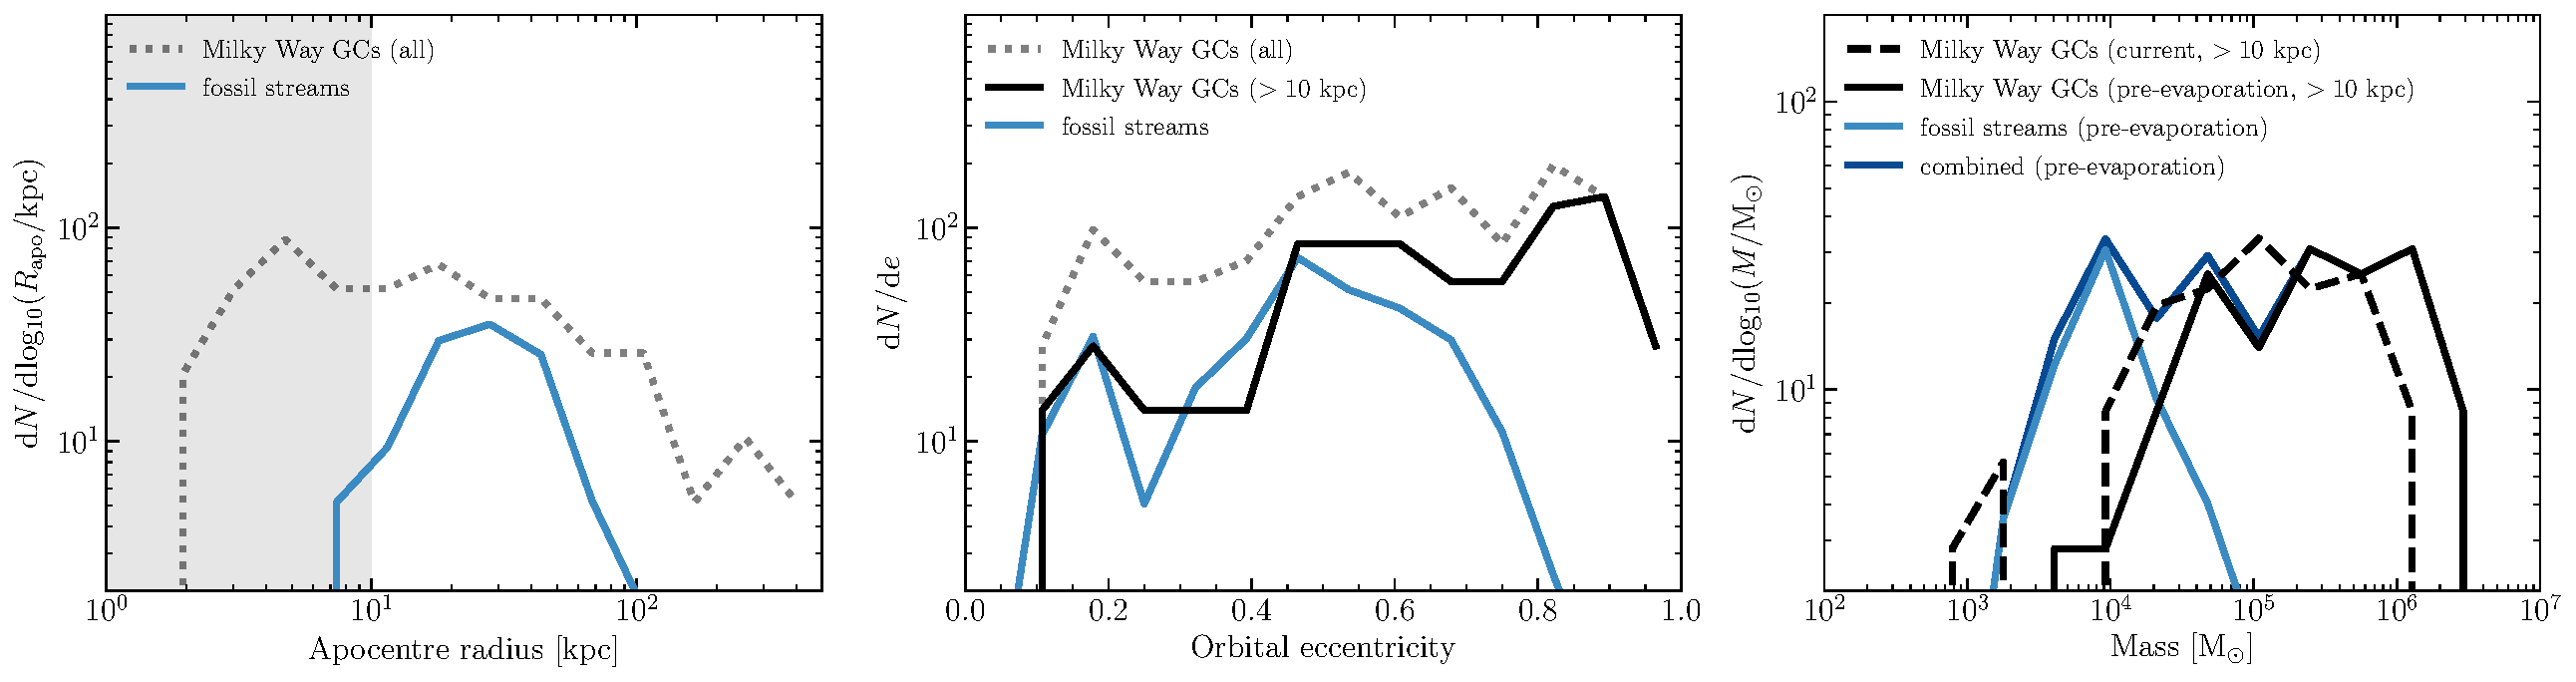
\includegraphics[width=\hsize]{distributions_mc.pdf}%
\caption{
\label{fig:hist}
Demographics of fossil streams (and their progenitor clusters) compared to those of the Galactic globular cluster population. Left: Apocenter radius distributions. The gray-shaded area indicates the inner radii ($\leq10$~kpc) where few fossil streams are found. In the middle and right panels, we therefore consider the globular clusters outside of these radii. Middle: Orbital eccentricity distributions. Globular clusters have an excess of high eccentricities ($e>0.5$) relative to fossil streams. Right: Mass distributions, both for current globular clusters and for the masses of fossil streams and globular clusters after rewinding their evaporation-driven mass loss in the Galactic halo. The progenitors of fossil streams were systematically a factor of 10--100 less massive than globular clusters.}
\end{figure*}	
We propagate the uncertainties on the fossil streams' orbital parameters into those on the pre-evaporation masses by applying eq.~(\ref{eq:m0}) to the entire sample of MCMC solutions. The resulting distributions of all apocenter radii, eccentricities, and pre-evaporation masses of the fossil streams in the MCMC sample are shown in \autoref{fig:hist}, where we also include the demographics of Galactic globular clusters that have survived till the present day \citep[2010 edition]{harris96}. For these surviving globular clusters, we also include an estimate of their pre-evaporation masses.

\autoref{fig:hist} reveals interesting differences between the demographics of fossil streams and globular clusters.
First, there is a distinct dearth of streams with apocenter radii $\leq10$~kpc.
We attribute this to incompleteness, as it is more challenging to identify streams within the solar circle.
Additionally, streams may have short lifetimes at small radii due to their short orbital periods.
For this reason, we exclude globular clusters with apocenter radii $\leq10$~kpc in the subsequent panels.
At larger radii, the streams follow approximately the same apocenter radius distribution as globular clusters, even if there may be a deficit of streams with apocenter radii $\geq60$~kpc.
This could again be related to completeness, because the photometric and kinematic detection of streams is more challenging at larger distances.
Second, we find that the eccentricity distribution of streams falls well below the distribution of globular clusters at large eccentricities.
This result is somewhat counterintuitive, because globular clusters on eccentric orbits are expected to be disrupted more rapidly (see equation~\ref{eq:t0}).
Rather than being the result of cluster disruption, we expect the difference in eccentricity distributions to result from the rapid disruption of fossil streams on plunging, eccentric orbits.
A strongly decreased lifetime of streams with high eccentricities could naturally produce the observed difference.

Finally, and most interestingly, the pre-evaporation masses of fossil streams and globular clusters differ significantly.
The median pre-evaporation mass of fossil streams is just $8.5\times10^3~\msun$, compared to $5\times10^5~\msun$ for globular clusters (and $1.5\times10^5~\msun$ for the current globular cluster masses).
This factor-of-60 difference in pre-evaporation mass directly reflects the fundamentally different nature of both classes of objects.
Globular clusters must have had the right properties to enable their survival over nearly a Hubble time, whereas fossil streams were disrupted by definition.
Since the orbital distributions only show mild differences when limiting the sample to apocenter radii $>10$~kpc, the pre-evaporation mass determines almost entirely whether a cluster survives as a globular cluster or results in a fossil stream.

\begin{figure*}
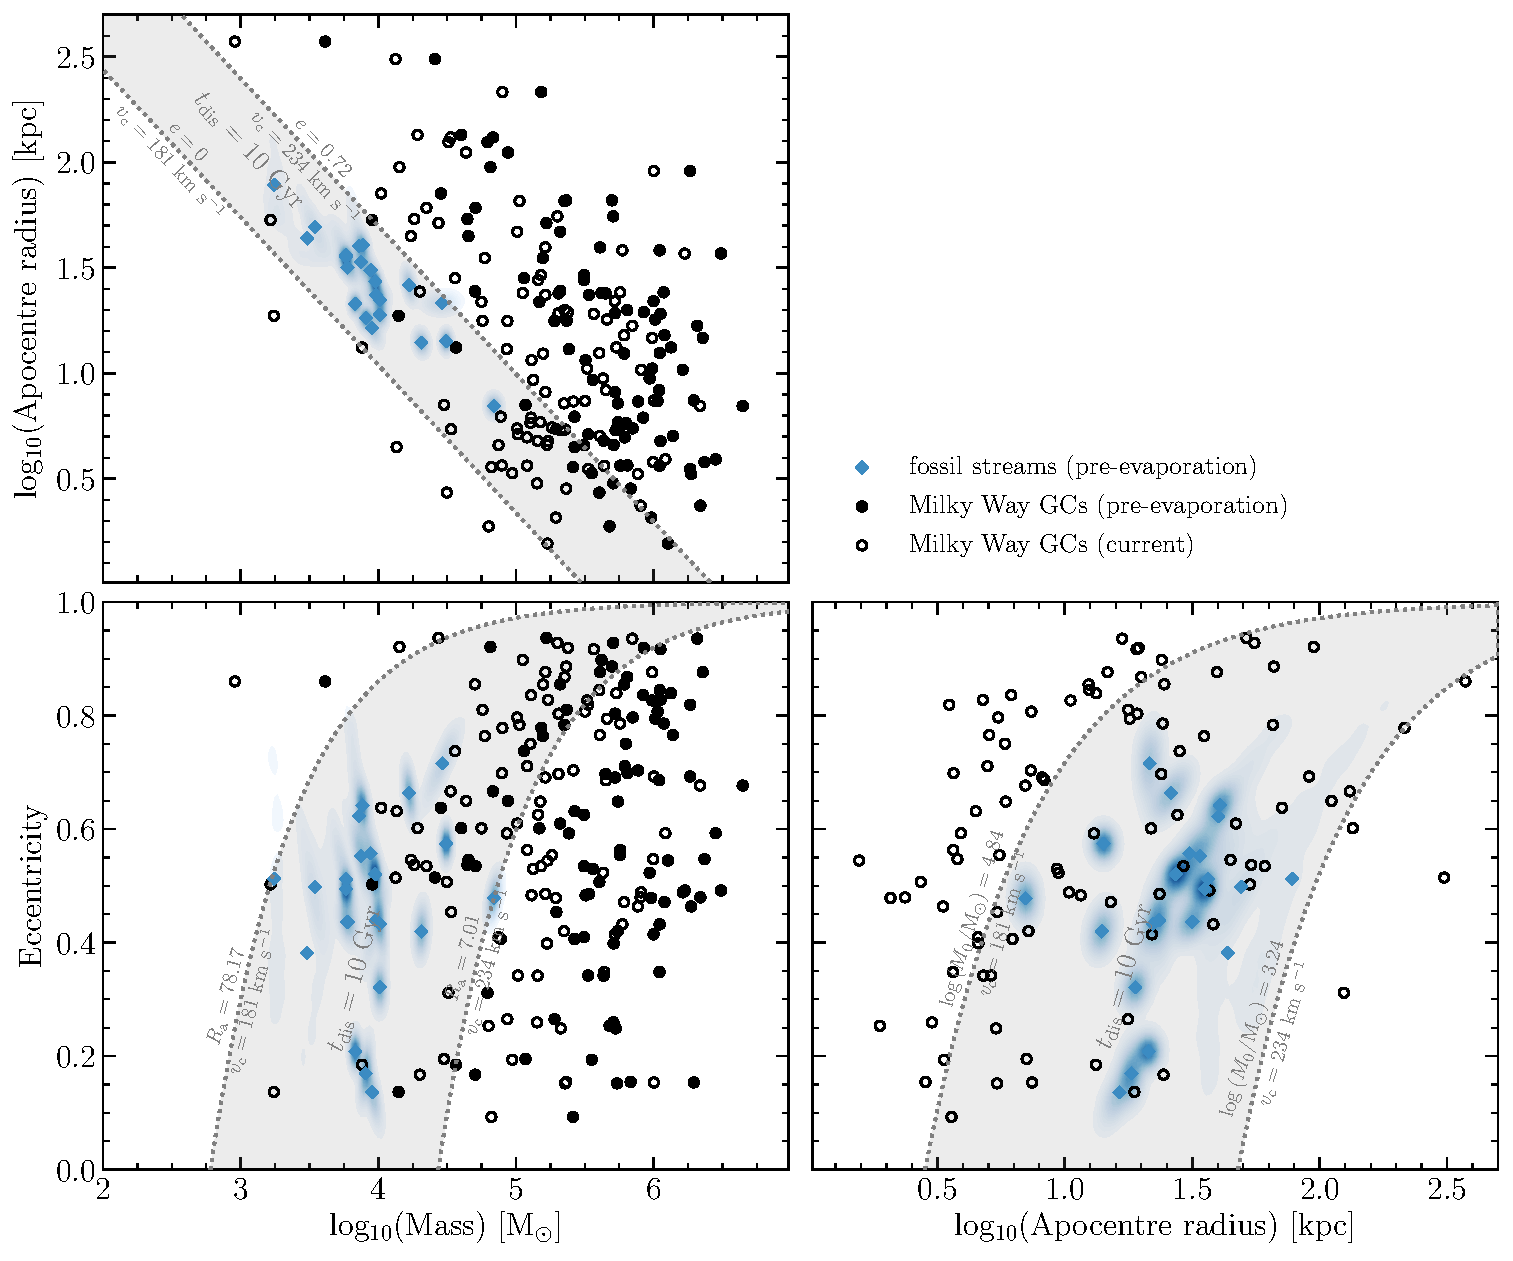
\includegraphics[width=\hsize]{distributions_2d_mc.pdf}%
\caption{
\label{fig:kde}
Two-dimensional demographics of fossil stream progenitors compared to those of the Galactic globular cluster population.
Top left: Mass-apocenter radius plane. Bottom left: Mass-eccentricity plane. Bottom right: Apocenter radius-eccentricity plane.
In each panel, the contours show a two-dimensional Gaussian kernel density estimate for the fossil stream progenitors, using the complete sample of MCMC realizations. 
Blue symbols show the best-fitting result for each fossil stream.
Open black symbols show current globular clusters, whereas filled black symbols show their pre-evaporation masses, i.e.\ those corrected for evaporation-driven mass loss on their current orbits.
In each panel, the gray-shaded band shows the range in each panel that is predicted to be occupied by the fossil stream progenitors assuming the evaporated over 10~Gyr of evolution, given their range of best-fitting orbital properties and progenitor masses (indicated by the annotations in gray).
The fossil stream progenitors are clearly offset from the globular clusters, especially in terms of their pre-evaporation masses (shown in the left-hand panels).}
\end{figure*}

\autoref{fig:kde} shows the two-dimensional projections of the same quantities as in \autoref{fig:hist}, together with the region within which clusters are predicted to be disrupted within 10~Gyr for the observed stream properties.
As expected, the streams fall within this region, which is systematically offset from the distributions of globular clusters, irrespectively of whether we adopt current or pre-evaporation globular cluster masses.
Stream progenitors had lower masses (which is necessary to end up as a stream at the present day), have somewhat lower eccentricities (because streams with high eccentricities are disrupted at pericenter), and occupied larger radii (because streams at small radii are difficult to observe and may survive less long).

Interestingly, the difference in apocenter radii manifests itself most strongly at low eccentricities.
It is well known that the orbits of globular clusters become radially anisotropic towards larger radii \citep[e.g.][]{dinescu99}, and the bottom right panel of Figure~\ref{fig:kde} shows that globular clusters with small apocenters have smaller eccentricities than those with large apocenters.
In contrast, there are no low-eccentricity fossil streams with small apocenters.
We expect this difference to be driven by the lack of searches for stellar streams towards the Galactic center \citep[e.g.,][]{malhan:2018, ibata:2019}, and faster disruption of stellar streams in the inner Galaxy \citep[e.g., due to enhanced dispersal caused by the rotating bar,][]{price-whelan:2016, hattori:2016}.
Finally, the top-left panel of \autoref{fig:kde} shows that the lack of streams with small apocenter radii limits their possible pre-evaporation masses to $<3\times10^5~\msun$. However, this is not responsible for the mass offset that we find. Even when extrapolating the expected distribution of the stream sample along the gray band to same range of apocenter radii as globular clusters, the pre-evaporation masses of streams remain about an order of magnitude lower than those of globular clusters.


\section{Summary and Discussion}
\label{sec:discussion}

We determined orbits of 22 disrupted Milky Way satellites by fitting sky positions, distances, and proper motions of the remnant stellar streams.
Assuming that the progenitors are globular clusters that evaporated recently, we integrated the orbit-dependent mass-loss rate to infer their pre-evaporation masses.
Surprisingly, the orbital distribution of disrupted globular clusters, in particular their apocenters and eccentricities, is similar to the orbital properties of the surviving population, even if there is a deficit of eccentricities $e>0.5$.
Most strikingly, the inferred masses of disrupted globular clusters peak at $8.5\times10^3\,\msun$ -- over an order of magnitude lower than the mass of a typical globular cluster in the Milky Way today, and a factor of $\sim60$ below the median pre-evaporation mass of surviving globular clusters.
In this section we discuss the implications of this population of low-mass, disrupted globular clusters for (globular) cluster formation (\S\,\ref{sec:discuss_gcform}), Galactic dynamics and assembly (\S\,\ref{sec:discuss_dynamics}), and early galaxy formation (\S\,\ref{sec:discuss_galform}).

\subsection{Formation mechanism of globular clusters}
\label{sec:discuss_gcform}
Our finding that the masses of stellar stream progenitors are lower than those of still bound clusters supports the picture in which globular clusters are the massive end of regular star cluster formation, rather than formed via a separate channel.
Because low-mass clusters are more susceptible to disruption than massive clusters \citep[e.g.,][]{fall:2001,kruijssen15b,reinacampos18}, today they are seen as stellar streams, whereas the more massive objects remain bound.
Even though the stream progenitors extend the globular cluster mass function to low masses, the combined distribution of pre-evaporation masses for stream progenitors and surviving clusters is still much shallower than the power-law mass function of young clusters observed today \citep[e.g.,][]{zhang:1999}.
If the initial mass function of globular clusters followed the same power-law distribution, this means that a large population of low-mass clusters remains unaccounted for.

In part, the comparative dearth of low-mass clusters may be attributed to the incompleteness of the stream sample and the finite lifetimes of the streams, but it may also signify that evaporation is a subdominant cluster disruption mechanism.
For example, \citet{kruijssen15b} proposed that most early-forming clusters were rapidly disrupted in the turbulent disks of their host galaxies, and that only a small fraction of the initial cluster population survives long enough to experience evaporation.
This phase of early disruption would shape the pre-evaporation demographics of the combined population of streams and globular clusters.
A complete census of stellar streams could therefore inform on dynamical properties of star-forming galaxies at high redshift.

Our results also have implications for the birth sites of globular clusters.
Specifically, the similarity in distributions of orbital apocenters and eccentricity between present-day globular clusters and fossil streams indicates that they have been predominantly accreted.
Most processes that destroy globular clusters operate more efficiently closer to the Galactic center \citep[e.g.,][]{gnedin:1997}.
Hence, if the initial population of globular clusters sampled the orbital space uniformly, we might expect to preferentially find stellar streams on more eccentric orbits with smaller apocenters.
However, streams from our sample occupy similar orbital families as the present-day globular clusters, and the main difference between the two populations is the lower average mass of disrupted clusters.
This may indicate that most globular clusters that ever orbited the Milky Way can be associated with a handful of its progenitor galaxies, in agreement with the phase-space \citep{massari:2019,trujillogomez20} and age-metallicity \citep{kruijssen19e,kruijssen20} distributions of the surviving cluster population.
Partly, streams with small apocenters and those with high eccentricities may be missing from our sample due to observational biases: low eccentricity tidal debris is more readily identifiable as a thin stellar stream \citep{hendel:2015}, while searching for streams in the inner Galaxy is challenging due to high contamination from the field Milky Way stars \citep[e.g.,][]{ibata:2019}.
The wealth of observational data expected over the next decade will allow for a more complete census of stellar streams that can further test the emerging picture in which the initial population of Galactic globular clusters originates from a small number of host galaxies.

\begin{figure}
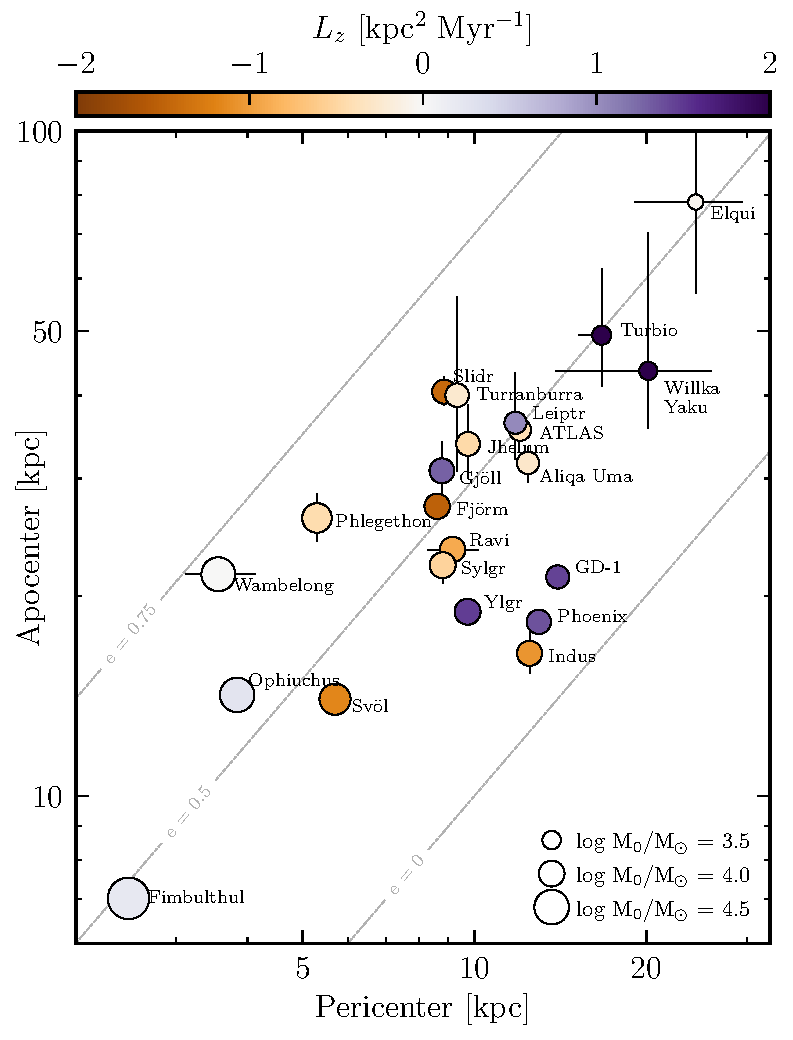
\includegraphics[width=\hsize]{streams_peri_apo.pdf}
\caption{
Apocenter versus pericenter of stellar streams' orbits:
orange for prograde ($L_z<0$), purple for retrograde ($L_z>0$), and white for radial orbits ($L_z\approx0$).
Error bars enclose the $16-84$ percentiles of the uncertainty range and dotted lines trace orbits of same eccentricity.
Larger symbols correspond to more massive progenitors, showing that streams in stronger tidal fields have preferentially higher pre-evaporation masses.
Similarities in orbital pericenters, apocenters, and angular momenta indicate that some streams might be dynamically associated.
}
\label{fig:individual_summary}
\end{figure}


\subsection{Dynamics of stellar streams}
\label{sec:discuss_dynamics}
Stellar streams are accurate tracers of the underlying gravitational potential \citep{bh:2018}.
In this section we discuss how derived orbits and masses inform us on the role of the progenitor globular cluster, its birth galaxy, and the Milky Way in shaping the detected tidal debris, ultimately improving our understanding of the streams' orbital histories in the Galaxy.

Orbital properties of individual streams in our sample are summarized in Figure~\ref{fig:individual_summary}, which shows their apocenters versus pericenters, as well as the $z$-component of their orbital angular momenta and the pre-evaporation mass.
In general, we infer higher masses for disrupted clusters that have orbited in stronger tidal fields: at a fixed eccentricity, streams on orbits with smaller apocenters have more massive progenitors.
Similarly, for a given apocenter radius, streams on more eccentric orbits have more massive progenitors.
The strong correlation between derived stream orbits and the pre-evaporation cluster masses is set in part because we assumed that all clusters have been dissolving for the same amount of time.
Future independent constraints on the streams' dynamical ages, for example from their phase-space dispersal \citep{buckley:2019}, could modulate this behavior by $<0.1$~dex in pre-evaporation mass (see \S\ref{sec:disrupted}).

Stellar streams may extend beyond their current detection limits at a lower surface brightness, so if they truly are disrupted globular clusters, we expect the pre-evaporation progenitor masses we derived here to be larger than their cumulative stellar masses.
However, the pre-evaporation masses of three streams in our sample (Elqui, Indus, and Jhelum) are an order of magnitude lower than their directly measured stellar masses \citep{shipp:2018}.
Recently, high-resolution spectroscopy showed these streams have abundance spreads consistent with low-mass dwarf galaxies \citep{ji:2020}, indicating that inferring a pre-evaporation mass lower than the observed stream mass means the stream is a disrupted dwarf galaxy rather than a globular cluster.
On the other hand, a pre-evaporation mass much larger than the detected stream stellar mass indicates significant portions of the debris remain undiscovered.
In the inner Galaxy, the high pre-evaporation masses of diffuse and short streams like Fimbulthul and Ophiuchus may signal enhanced dispersal of tidal debris, for example, due to the dynamical influence of the rotating Galactic bar \citep{hattori:2016, price-whelan:2016}.
In the outer Galaxy, however, we also find that the pre-evaporation masses of Phoenix and Wambelong are $\approx2.5$ and $10$ times larger than their respective stellar masses \citep{shipp:2018}.
According to our orbital constraints, these streams are close to their apocenter, so the missing stellar mass is likely due to observational limitations, and may be recovered in deeper data.
Finally, the directly measured stellar masses of the following streams agree well with the pre-evaporation masses we inferred, indicating they likely have been mapped in full: the Aliqa Uma--ATLAS complex, Ravi, Turbio, Turranburra, and Willka Yaku.
Our assurance that the entire system has been observed will aid the construction of dynamical models that reproduce the observed streams.

Interestingly, Figure~\ref{fig:individual_summary} shows that several groups of streams have similar pericenters, apocenters, and angular momenta.
Different streams can have similar orbits because: (1) they were originally part of the same stream, as recently reported for ATLAS and Aliqa Uma \citep{li:2020}, or (2) they were accreted in the same host dwarf galaxy, as suggested for GD-1 and Kshir \citep{malhan:2019}.
In our sample, ATLAS and Aliqa Uma have the most similar orbits, and their combined stellar mass agrees well with the pre-evaporation mass we inferred for their respective progenitors, adding further evidence they are debris from the same globular cluster progenitor.
Very retrograde and with large apocenters, $\approx45\,\kpc$, Turbio and Willka-Yaku form a loose group, as do GD-1, Phoenix, and Ylgr at smaller apocenters, $\approx20\,\kpc$, and more mildly retrograde orbits.
These groups are more likely to be evidence of group infall.
Another stream, Hermus (not included in our analysis due to the lack of proper motions), may be associated with the latter group, as \citet{grillmair:2016} showed that in projection it lies close to the orbit of the Phoenix stream.
Improved proper motions from future Gaia data releases and orbit integrations in more realistic, time-dependent Milky Way models \citep[e.g., those that self-consistently include Large Magellanic Cloud and Sagittarius,][]{petersen:2020, garavito-camargo:2020, vasiliev:2020} will test the nature of these stream associations.

Finally, we examine how the inferred progenitor masses affect stellar streams as detectors of dark-matter substructure.
Numerical simulations show that a low-mass dark-matter subhalo encountering a stellar stream can kinematically heat the stream and produce an under-density (gap) at the location of closest approach \citep[e.g.,][]{johnston:2002, ibata:2002, carlberg:2009, yoon:2011, erkal:2015}.
However, patterns of under- and over-densities naturally arise in stellar streams due to epicyclic pile-ups of stars \citep[e.g.,][]{kupper:2008, just:2009, kupper:2010}.
Recently, density variations were discovered in the GD-1 stream \citep{pwb, deboer:2020}, and both external perturbation \citep{bonaca:2019b, banik:2019} and epicycles \citep{ibata:2020} have been invoked as their origin.
More massive globular clusters imprint stronger epicyclic variations, so an accurate accounting of the stream progenitor's mass would constrain the amount of density variation that can be attributed to epicycles.
We find that the GD-1 progenitor of $\approx7\times10^3\,\msun$ was slightly less massive than assumed in modeling so far ($7\times10^4\,\msun$ by \citealt{bonaca:2019b}, and $3\times10^4\,\msun$ by \citealt{ibata:2020}).
Our measurements of pre-evaporation masses provide an opportunity to construct more realistic models of streams like the GD-1, and ultimately put more stringent limits on the abundance of dark-matter subhalos in the Milky Way.



\subsection{Early galaxy formation}
\label{sec:discuss_galform}
We can place the pre-evaporation masses of the progenitor clusters in the context of their formation environment by assuming that at birth they had the same metallicity as their host galaxy, and using the metallicity of the stream to infer the galaxy mass at the time of cluster formation \citep{kruijssen20b}. This is possible, because the galaxy mass-metallicity relation is predicted to exhibit little evolution over the formation redshift range of the metal-poor clusters considered here, such that the stream metallicity mostly traces the natal galaxy mass, rather than the formation redshift. Metallicities are available for nine of the streams in our sample (Aliqa Uma, ATLAS, Fj\"orm, GD-1, Ophiuchus, Phoenix, Slidr, Sylgr, and Ylgr; \citealt{ibata:2019,li:2020,wan20}). We follow \citet{kruijssen19c} and convert these metallicities to natal galaxy masses using the galaxy mass-metallicity relation between $z=3$ and $z=6$ predicted by the FIRE simulations \citep{ma16}.

\begin{figure}
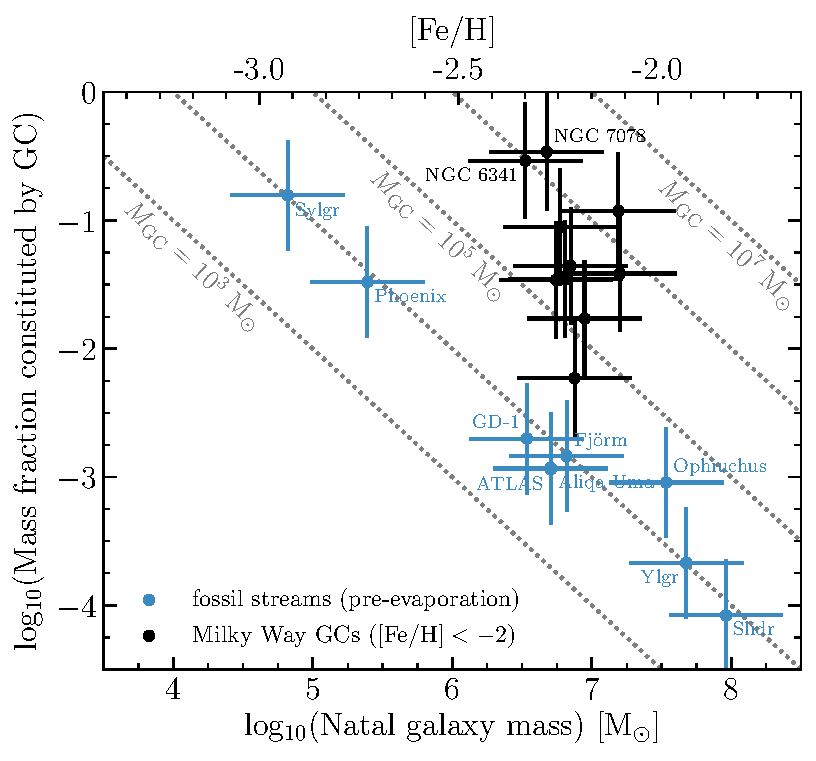
\includegraphics[width=\hsize]{mhost_fraction.pdf}
\caption{
\label{fig:mhost}
Mass fraction of the natal galaxy constituted by the progenitors of fossil streams (blue) and low-metallicity globular clusters (black) as a function of the galaxy mass.
The sample is restricted to fossil streams with known metallicities, which are converted to a natal galaxy mass using the galaxy mass-metallicity relation between $z=3$ and $z=6$.
Error bars combine metallicity uncertainties with the evolution of the mass-metallicity relation across this redshift range.
On average, stream progenitors constituted a smaller fraction of their natal galaxy's mass than globular clusters, but the progenitors of the most metal-poor streams likely represented a significant fraction of the lowest-mass galaxies ever to exist.
}
\end{figure}

\autoref{fig:mhost} shows the resulting relation between the galaxy mass fraction constituted by the stream progenitor clusters (using their pre-evaporation masses) and the natal galaxy mass.
For comparison, we are also including the ten GCs with metallicities $[{\rm Fe}/{\rm H}]<-2$ from the compilation of \citet{kruijssen19e}.
The ranges of pre-evaporation masses of streams ($10^{3.7}{-}10^{4.5}~\msun$) and globular clusters ($10^{4.6}{-}10^{6.3}~\msun$) are each considerably narrower than the total range of natal galaxy masses ($10^{4.8}{-}10^{8.0}~\msun$).
As a result, the galaxy mass fraction constituted at birth is controlled primarily by the natal galaxy mass, such that the fraction decreases with galaxy mass and metallicity.
The typical mass fraction constituted by stream progenitors must have been of the order $10^{-3}$ (due to their low masses), whereas it was typically a few percent for the metal-poor GCs considered here. The two very most metal-poor GCs (NGC~6341 and NGC~7078) may have constituted anywhere between 10--100\% of their host galaxies.

Due to the narrow range of stream masses, their metallicity is a strong predictor for the galaxy mass fraction they constituted at birth.
The highest fractions are found at the lowest metallicities.
The recently-measured metallicity of the Phoenix stream \citep{wan20} implies that its progenitor cluster represented $3.3_{-2.1}^{+5.7}$\% of its host galaxy at formation, whereas we estimate that the progenitor of the extremely metal-poor Sylgr stream \citep{ibata:2019,roederer:2019} constituted $16_{-10}^{+27}$\% of its host galaxy.
This means that the progenitors of fossil streams below the GC `metallicity floor' \citep{beasley:2019,kruijssen19c} of $[{\rm Fe}/{\rm H}]\approx-2.5$ may have represented a relevant fraction of the host galaxy mass, ranging anywhere from 1--100\%.
These host systems were the lowest-mass galaxies ever to exist, with $<10^6~\msun$.
Individual stream progenitors may have had a profound impact on the early formation of these host galaxies and potentially their reionization.
In future observations of galaxies with stellar masses $\la10^6~\msun$ with the JWST, such progenitor clusters should manifest themselves as bright knots \citep[e.g.][]{pfeffer19}.
These systems should not survive as GCs, because they would fall below the GC metallicity floor observed at $z=0$ \citep[except under rare circumstances, see][]{larsen20}, but they would be potential stream progenitors.
Such high-redshift observations would directly connect the galactic archaeological results presented in this paper to direct observations of the young stellar systems in their birth environments.


\vspace{0.5cm}
\acknowledgements
It is a pleasure to thank Sownak Bose, M\'{e}lanie Chevance, and Charlie Conroy for helpful discussions.
AB acknowledges support from NASA through HST grant HST-GO-15930.
J.M.D.K.\ gratefully acknowledges the generous hospitality of the Institute for Theory and Computation at Harvard University, where this work was instigated and part of it was carried out. J.M.D.K.\ gratefully acknowledges funding from the Deutsche Forschungsgemeinschaft (DFG, German Research Foundation) through an Emmy Noether Research Group (grant number KR4801/1-1) and the DFG Sachbeihilfe (grant number KR4801/2-1), as well as from the European Research Council (ERC) under the European Union's Horizon 2020 research and innovation programme via the ERC Starting Grant MUSTANG (grant agreement number 714907).

\software{
\package{Astropy} \citep{astropy, astropy:2018},
\package{gala} \citep{gala},
\package{IPython} \citep{ipython},
\package{matplotlib} \citep{mpl},
\package{numpy} \citep{numpy},
\package{scipy} \citep{scipy}
}

\appendix
\section{The origin of stream data and resulting orbital constraints}
\label{sec:appendix}
The stream data that we fit in this work can be separated into three categories: 1) sky positions and proper motions, 2) heliocentric distance, and 3) radial velocities.
In the right-most column of Table~\ref{table:phasespace}, we report references for each stream in these categories.
Sky positions and proper motions are reported for individual member stars in most of the streams \citep[e.g.,][]{ibata:2019, shipp:2019}. However, for GD-1 we use average properties along the stream track \citep{pwb}, and for Ravi, Turbio, Wambelong, and Willka-Yaku we use the reported orbital poles and the average proper motions \citep{shipp:2019}.
We use average distance to the stream at its end-points summarized in \citet{riley:2020}, with the exception of GD-1, where we use the distance gradient from \citet{koposov:2010}, and Ophiuchus, where we use the distance gradient inferred by \citet{sesar:2015}.
Radial velocities are missing for most of the streams in our sample (marked as `N/A' in Table~\ref{table:phasespace}), but we use individual measurements for Ophiuchus from \citet{caldwell:2020}, GD-1 from \citet[which includes data from \citealt{koposov:2010} and \citealt{huang:2019}]{bonaca:2020b}, and average radial velocity trends reported for Aliqa Uma and ATLAS in \citet{li:2020}.

These data are used to constrain the streams' orbits.
As described in Section~\ref{sec:orbits}, we parameterize each orbit with a set of five phase-space parameters at a fixed right ascension.
Columns 2--7 of Table~\ref{table:phasespace} provide the control R.A.\ and phase-space coordinates derived in our fiducial model of the Milky Way.
For each of the orbital parameters, we provide the median of the sampled posterior distribution and the $16-84$ percentile uncertainties.
Orbital declination, distance, and proper motions have been constrained very precisely for all of the streams thanks to the wealth of observational data.
In some streams, the 5D observables put strong constraints on the orbit, so the allowed uncertainties in radial velocity are also small (e.g., Fj\" orm, Sylgr).
However, for many streams the addition of radial velocities would significantly improve the orbital constraints.

\begin{deluxetable}{l @{\hspace{0.5cm}} c D D D D D c}
\tablehead{
Name & R.A. & \multicolumn2c{Dec} & \multicolumn2c{distance} & \multicolumn2c{$\mu_\alpha$} & \multicolumn2c{$\mu_\delta$} & \multicolumn2c{$V_r$} & Data\\
& deg & \multicolumn2c{deg} & \multicolumn2c{kpc} & \multicolumn2c{\masyr} & \multicolumn2c{\masyr} & \multicolumn2c{\kms} & references
}
\decimals
\setlength{\tabcolsep}{3pt}
\startdata
Aliqa Uma & $31.0$ & -32.11$^{+0.11}_{-0.11}$ & 18.60$^{+1.46}_{-1.67}$ & 0.16$^{+0.02}_{-0.02}$ & -0.76$^{+0.03}_{-0.04}$ & -52.20$^{+1.48}_{-1.50}$ & [1, 2, 3]\\ 
ATLAS & $9.0$ & -20.62$^{+0.09}_{-0.09}$ & 16.80$^{+0.36}_{-0.36}$ & -0.62$^{+0.02}_{-0.03}$ & -0.96$^{+0.02}_{-0.02}$ & -145.40$^{+1.34}_{-1.30}$ & [1, 2, 3]\\ 
Elqui & $10.0$ & -36.68$^{+0.32}_{-0.33}$ & 49.09$^{+6.00}_{-5.37}$ & 0.05$^{+0.05}_{-0.06}$ & -0.44$^{+0.03}_{-0.03}$ & -101.40$^{+153.83}_{-143.78}$ & [1, 2, N/A]\\ 
Fimbulthul & $198.0$ & -28.64$^{+0.08}_{-0.08}$ & 4.45$^{+0.05}_{-0.05}$ & -9.06$^{+0.11}_{-0.11}$ & -8.10$^{+0.09}_{-0.09}$ & 246.92$^{+4.72}_{-4.75}$ & [4, 2, N/A]\\ 
Fj\"{o}rm & $260.0$ & 66.20$^{+0.07}_{-0.06}$ & 5.56$^{+0.06}_{-0.07}$ & 4.82$^{+0.13}_{-0.14}$ & 2.88$^{+0.07}_{-0.07}$ & -31.14$^{+2.35}_{-2.17}$ & [4, 2, N/A]\\ 
GD-1 & $123.0$ & -10.50$^{+0.16}_{-0.16}$ & 8.78$^{+0.05}_{-0.06}$ & -1.33$^{+0.01}_{-0.01}$ & -8.57$^{+0.05}_{-0.05}$ & 298.57$^{+0.70}_{-0.73}$ & [5, 5, 6]\\ 
Gj\"{o}ll & $90.0$ & -20.50$^{+0.11}_{-0.11}$ & 3.22$^{+0.07}_{-0.07}$ & 23.99$^{+0.21}_{-0.23}$ & -22.43$^{+0.20}_{-0.19}$ & 169.97$^{+7.95}_{-7.57}$ & [4, 2, N/A]\\ 
Indus & $352.0$ & -63.80$^{+0.17}_{-0.16}$ & 14.04$^{+0.34}_{-0.26}$ & 4.35$^{+0.03}_{-0.03}$ & -4.42$^{+0.04}_{-0.04}$ & -9.93$^{+4.86}_{-4.56}$ & [1, 2, N/A]\\ 
Jhelum & $4.0$ & -52.22$^{+0.25}_{-0.26}$ & 11.59$^{+0.35}_{-0.31}$ & 8.01$^{+0.03}_{-0.03}$ & -3.45$^{+0.03}_{-0.03}$ & 21.58$^{+5.16}_{-4.42}$ & [1, 2, N/A]\\ 
Leiptr & $98.0$ & -34.94$^{+0.11}_{-0.11}$ & 7.12$^{+0.24}_{-0.19}$ & 10.10$^{+0.15}_{-0.14}$ & -8.15$^{+0.10}_{-0.11}$ & 268.22$^{+7.76}_{-7.20}$ & [4, 2, N/A]\\ 
Ophiuchus & $240.5$ & -7.35$^{+0.01}_{-0.01}$ & 9.90$^{+0.02}_{-0.02}$ & -4.21$^{+0.03}_{-0.03}$ & -4.57$^{+0.01}_{-0.00}$ & 275.69$^{+0.43}_{-0.38}$ & [7, 7, 7]\\ 
Phlegethon & $299.0$ & -62.69$^{+0.25}_{-0.25}$ & 4.60$^{+0.07}_{-0.07}$ & -10.03$^{+0.07}_{-0.08}$ & -20.40$^{+0.14}_{-0.18}$ & 357.07$^{+6.85}_{-6.38}$ & [8, 2, N/A]\\ 
Phoenix & $27.5$ & -43.75$^{+0.08}_{-0.08}$ & 16.41$^{+0.16}_{-0.15}$ & 2.74$^{+0.03}_{-0.03}$ & -0.08$^{+0.02}_{-0.02}$ & 31.16$^{+9.87}_{-9.58}$ & [1, 2, N/A]\\ 
Ravi & $344.1$ & -60.87$^{+0.29}_{-0.30}$ & 25.72$^{+1.19}_{-1.21}$ & 0.97$^{+0.06}_{-0.06}$ & -2.71$^{+0.15}_{-0.16}$ & 38.73$^{+32.38}_{-25.98}$ & [1, 2, N/A]\\ 
Slidr & $148.0$ & 14.04$^{+0.10}_{-0.10}$ & 2.77$^{+0.03}_{-0.03}$ & -27.71$^{+0.27}_{-0.27}$ & -8.58$^{+0.12}_{-0.12}$ & -32.54$^{+4.53}_{-4.96}$ & [4, 2, N/A]\\ 
Sv\"{o}l & $250.0$ & 24.15$^{+0.12}_{-0.13}$ & 7.77$^{+0.13}_{-0.14}$ & 2.75$^{+0.17}_{-0.15}$ & -6.34$^{+0.13}_{-0.13}$ & -97.65$^{+12.29}_{-13.46}$ & [4, 2, N/A]\\ 
Sylgr & $164.0$ & -10.90$^{+0.09}_{-0.10}$ & 2.50$^{+0.04}_{-0.04}$ & -23.63$^{+0.21}_{-0.22}$ & -22.47$^{+0.18}_{-0.21}$ & -59.92$^{+4.20}_{-4.57}$ & [4, 2, N/A]\\ 
Turbio & $27.8$ & -45.12$^{+2.27}_{-2.04}$ & 15.86$^{+0.79}_{-0.73}$ & 2.05$^{+0.10}_{-0.10}$ & 1.89$^{+0.25}_{-0.28}$ & 64.19$^{+75.56}_{-80.66}$ & [1, 2, N/A]\\ 
Turranburra & $59.0$ & -18.41$^{+0.25}_{-0.22}$ & 15.77$^{+1.19}_{-1.20}$ & 0.30$^{+0.08}_{-0.07}$ & -1.22$^{+0.04}_{-0.04}$ & -89.68$^{+53.51}_{-52.47}$ & [1, 2, N/A]\\ 
Wambelong & $91.0$ & -46.60$^{+0.16}_{-0.15}$ & 16.05$^{+0.84}_{-0.74}$ & 2.19$^{+0.13}_{-0.13}$ & -1.52$^{+0.11}_{-0.10}$ & 164.77$^{+21.56}_{-23.36}$ & [1, 2, N/A]\\ 
Willka Yaku & $38.5$ & -57.88$^{+0.08}_{-0.09}$ & 34.45$^{+1.86}_{-1.87}$ & 1.16$^{+0.07}_{-0.07}$ & 0.35$^{+0.15}_{-0.16}$ & 123.42$^{+121.86}_{-126.02}$ & [1, 2, N/A]\\ 
Ylgr & $183.0$ & -36.79$^{+0.07}_{-0.07}$ & 10.44$^{+0.14}_{-0.14}$ & 0.26$^{+0.04}_{-0.04}$ & -5.90$^{+0.12}_{-0.11}$ & 300.33$^{+8.05}_{-7.25}$ & [4, 2, N/A]\\ 

\enddata
\caption{Constrained orbital parameters of stellar streams: declination, distance, proper motions and radial velocity at a control R.A. location.
Quoted values are the medians of the sampled posterior distributions and the uncertainties reflect their $16-84$ percentiles.
Last column gives the origin of the stream data (sky positions and proper motions, distance, radial velocity), with the following key: 1) \citet{shipp:2019}, 2) \citet{riley:2020}, 3) \citet{li:2020}, 4) \citet{ibata:2019}, 5) \citet{pwb}, 6) \citet{bonaca:2020b}, 7) \citet{caldwell:2020}, 8) \citet{ibata:2018}.
}
\label{table:phasespace}
\end{deluxetable}


\bibliographystyle{aasjournal}
\bibliography{disrupted_gc}


\end{document}


